\documentclass[12pt,a4paper]{report}
\usepackage{graphicx}
\usepackage{tabularx}
\usepackage{array}

\begin{document}
%--------------Title Page ------------------
\thispagestyle{empty}
\begin{center}
\textbf{\large{Merchant Monetary System}}\\
\vspace{0.5cm}
\textbf{ CS-262 Design Document} \\
\vspace{1.5cm}

\includegraphics[scale=.07]{UETLogo}\\
\vspace{1.5cm}
\underline{ Project Supervisor}\\
\vspace{0.5cm}
Mr. Samyan Qayyum Wahla\\
\vspace{1cm}
\underline {Group ID $(G 11)$} \\
\vspace{0.5cm}
Project Member\\
\vspace{0.5cm}
\begin{tabular}{c c c }
 Syed Hashir & 2021-CS-1 \\ 
 Kabir Ahmed & 2021-CS-4  \\  
 M. Hamad Hassan & 2021-CS-33
\end{tabular}
\vspace{2cm}
\par\rule{\textwidth}{0.5pt} 
Department of Computer Science\\
University of Engineering and Technology, Lahore\\
Pakistan
\end{center}
\newpage

\tableofcontents
\thispagestyle{empty}
\pagenumbering{arabic}


\newpage
\setcounter{page}{1}
\chapter {Project Description}

The system is designed for a company that provides:
Logistics (delivery of products to its client), product management (crud operations), and effective communication with their employee and clients.
 
The company has its office, warehouse, and rider. 
It has a different contract with multiple firms to take the shipment and store it in dedicated warehouses. The rider will take orders from the shopkeeper. Their order is received at the office, and the office will create the feasibility report according to their client's needs and instructions generated for their warehouse manager to fulfill their order. The available rider will receive an email about their order. The office will send a confirmation email to their client. 
 
There are a total of four actors in the system and one stakeholder. Their title and role are:
\begin{itemize}
\item \textbf{ CEO:} The owner of the company could manage all the operations.
\item \textbf{Employee:} They directly report to CEO and help in company operations.  
\item \textbf{Warehouse Manager:} Ready the shipment for the rider and managed other expenses.
\item \textbf{Rider:} Received the order detail and delivered the product to pre-subscribed routes.
\end{itemize}
The stakeholder is:
\begin{itemize}
\item \textbf{Shopkeepers:} The rider will take the order from the shop owner and deliver it. The rider will receive all orders and payments.
\end{itemize}
All the actors will be able to create their accounts, and the system will give specific security codes to them. It helps to protect the system from security breaches.
 
There first dedicated dashboard for the owner where they monitor all operations. The operations manage their employees, products, and expenses and send emails. The CEO is the only person in the system with access to all operations. CEOs could analyze company operations, including the performance of their workers. The system will generate the company expenditure report.
 
The second dashboard is for the office employees directly contacting the CEO. They have access to manage emails, clients' orders, vendors' orders, and company expenses. The company's expenses are the CEO, rider, and warehouse salaries. The payment of the vendor and clients. An employee will enter all the shipments that the company receives their record. They add the product name, SKU number, weight, volume, cost price, manufacturer, and many more to identify confirmed products.
 
The third dashboard is for the warehouse manager, who receives feasibility reports of office employees and readies the order for the rider. The warehouse manager must record the labor used in preparing the order. It could provide the miscellaneous expenses of the warehouse, like electricity costs, etc. They can view the product and make suitable changes according to the requirements. 
 
The fourth dashboard is for a rider who takes orders from the warehouse and delivery them to the company client. The system will provide the routes for the destination with the order detail. The rider received a specific amount of fuel to perform the operations. The prescribed fuel is calculated according to the formula. They can see all the products. The product will be sorted in order, like assessing and descending. Search for a specific product from a wide range of available products. The system will deploy different sharp algorithms to access the desired date quickly. Able to place the order and view the detail of the order as well. The order is placed according to the stakeholder shopkeeper's needs.
 
The system will provide the report to the CEO according to the performance of their worker, expenditure, and profit.
Like how many products are received in the warehouse, how many products are left, how many products are delivered to company clients, how many riders have done shipments, which rider performs most shipments, and which rider needs to perform better. It also includes how many orders a shopkeeper placed and whether the company received the payment. 
 
The email notification mechanism is embedded in the system, which helps the company communicate within and outside with other vendors and clients. The internal communication will send the order details to the warehouse manager to prepare the shipment for the rider. The rider also received the email for the delivery of the order. The employee emails the CEO for any need of assistance with an issue. The warehouse manager and rider also mail to the company office for any assistance. In external communication, the client will receive a confirmation email from the system about their order. They also take assistance from the company with any issue.
 
The flow of new users will be like this. A potential user provides the required detail for account creation, and an employee or CEO selects their role in the company. A unique username is allowed to login into the system. Account successfully creation the, they create the security code to use the system according to their role. 
 
All the data is stored in an effective data structure to extract the data according to the need of the system actor and stakeholder


\newpage
\chapter {Project Features}

\begin{enumerate}
\item CEO are able to manage employee, warehouse manager, rider and shopkeeper.  
\item CEO and Employee manage product related operations.
\item CEO will be able to analyze company operations.  
\item Warehouse manager ready the shipment for rider. 
\item Rider delivered the shipment to their shopkeeper. 
\item Rider are able to selected the shortest route to reach the destination.  
\item One user is able to notify other user through email.
\item Rider are able to view products and place order. 
\item Dedicated security password for each user. 
\item Company expenditure report will be generated.

\end{enumerate}

\newpage
\chapter {Technology Stack}
The project is completed under following stack \\ 
\begin{tabularx}{0.9\textwidth} { 
  | >{\raggedright\arraybackslash}X 
  | >{\centering\arraybackslash}X |
  }
  \hline
 Language & C \# (.net framework 4.8)   \\
 \hline
IDEs  & Microsoft Visual Studio 2022  \\
\hline
\end{tabularx}
\newpage
\chapter {Project Actors}
The actors are:
\begin{itemize}
\item \textbf{ CEO:} The owner of company could manage all the operations.
\item \textbf{Employee:} They directly reported to CEO and help in company operations.    
\item \textbf{Warehouse Manager:} Ready the shipment for rider and manage other expenses. 
\item \textbf{Rider:} Received the detail of order and delivered the product to prescribed routes.  
\end{itemize}
The stakeholder is:
\begin{itemize}
\item \textbf{Shopkeepers:} Are able to outlook products, place order and check detail.
\end{itemize}
\newpage
\chapter {Use Cases}
%------------------------------------------
\section{Use Case 1(Log In)}
\begin{tabular}{ | m{3cm} | m{12cm}| } 
  \hline
Use Case ID & U01   \\\hline
Name  &  Login Screen \\ \hline
Actor &   CEO, Employee, Rider, Warehouse Manager \\ \hline
Description & Respected user will login to this system by providing valid role, username and password. After clicking on Login Button, System will check for its validity if this user is already exist on database. After successful validation, respected panel will show them.  \\ \hline
UI Interface in JUSTINMIND & \begin{center}
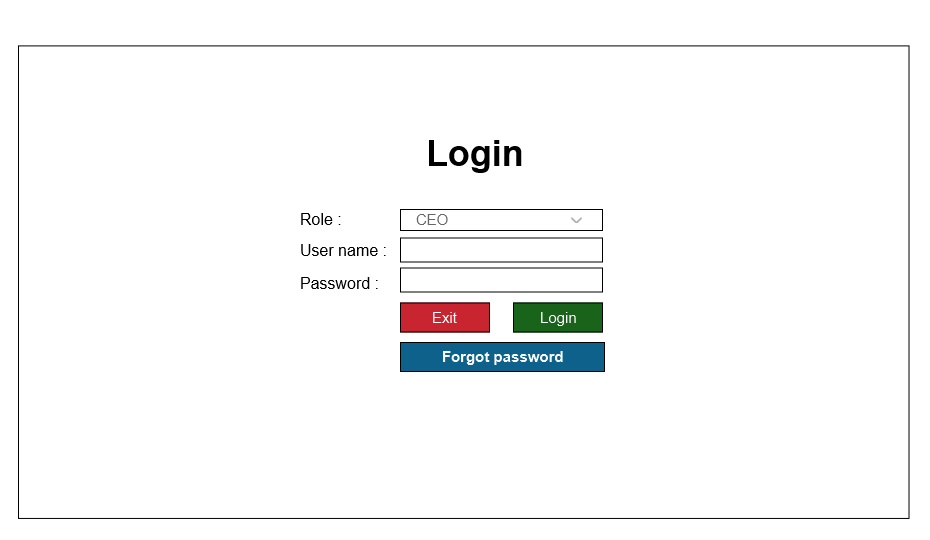
\includegraphics[scale=0.3]{./UIs for Latex Reports/UI-002 Login@1x.png}
\end{center}  \\ \hline
Pre-Condition & Respective User Will initiate this system.  \\ \hline

\end{tabular}
\newpage
\begin{tabular}{ | m{3cm} | m{12cm}| } 
\hline
Flow & Main Scenario:
\begin{enumerate}
\item   By Default Login Screen will appear first
\item	Select Your Role from combo box then.
\item	Provide your username you chose while signing up.
\item	Then enter password for your account
\item	Then Click on Login Button
\end{enumerate}
Alternate Flow:
\begin{itemize}
\item If forgot password button is clicked
	\begin{enumerate}
		\item Interface I02 will get open
	\end{enumerate}
\item If user provides invalid username and password
	\begin{enumerate}
	    \item	Message box with a message of invalid input will be displayed
		\item System remains on the same page
	\end{enumerate}
\item If user provides unregistered information
	\begin{enumerate}
		\item Message Box with a message of “User Not Found” will get displayed
	\end{enumerate}
\item If user don’t provide all required information
	\begin{enumerate}
		\item Alert Message will be displayed.
	\end{enumerate}
\item If Exit Button is Clicked  
\end{itemize}
\\ \hline
Post-Condition & Password will successfully changed  \\ \hline

\end{tabular}
%------------------------------------------
\section{ }

\begin{tabular}{ | m{3cm} | m{12cm}| } \hline

Use Case ID &   \\\hline

Name  	    &   \\ \hline

Actor     	&  \\ \hline

Description &  \\ \hline

UI Interface in JUSTINMIND & \begin{center} 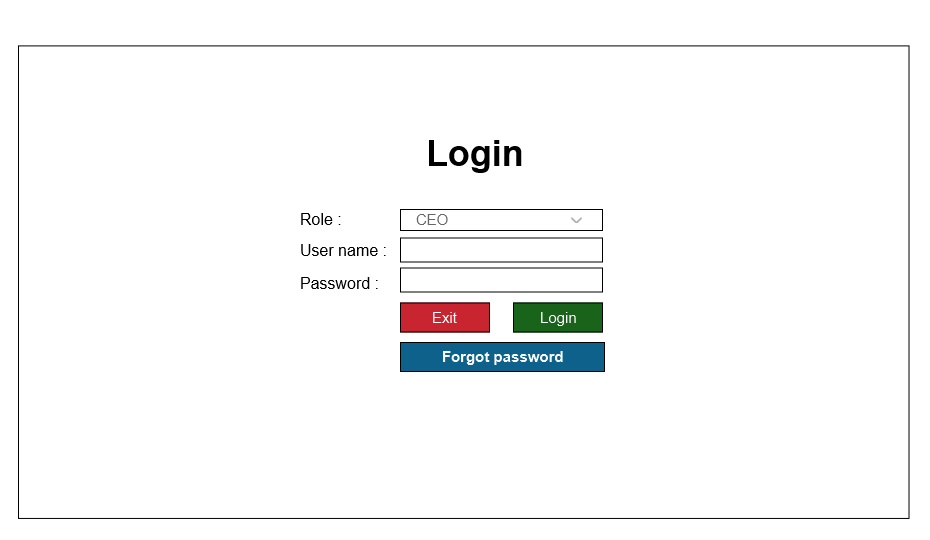
\includegraphics[scale=0.3]{./UIs for Latex Reports/UI-002 Login@1x.png}\end{center}  \\ \hline

Pre-Condition &   \\ \hline

\end{tabular} \newpage \begin{tabular}{ | m{3cm} | m{12cm}| }  \hline
Flow & Main Scenario:

\begin{enumerate}
\item   
\item	
\item	
\item	
\item
\end{enumerate}

Alternate Flow:

\begin{itemize}
\item
	\begin{enumerate}
		\item 
	\end{enumerate}
\item 
	\begin{enumerate}
	   	 \item	
		\item 
	\end{enumerate}
\item 
	\begin{enumerate}
		\item 
	\end{enumerate}
\item 
	\begin{enumerate}
		\item 
	\end{enumerate}
\item 
\end{itemize}
\\ \hline
Post-Condition &    \\ \hline

\end{tabular}
%------------------------------------------
















\end{document}



